\section{Validation of the TLP-HMM}

\subsection{Model validation}

The response of the generator is tested in conditions as close as possible to the ISO 10605 standard \cite{iso10605}.
The generator is connected to a 2\textOmega{} load, itself connected to a 12 GHz (10 ps/sample point) oscilloscope with a 50\textOmega{} input impedance.
The setup (Fig. \ref{fig:injection_setup_validation}) has the same loading impedance than the standard measurement target \cite{iso10605, iec61000-4-2}.

\begin{figure}[!h]
  \centering
  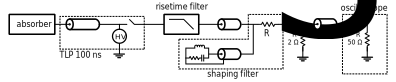
\includegraphics[width=0.9\textwidth]{src/5/figures/validation_injection_setup.pdf}
  \caption{Injection setup for validating the generator}
  \label{fig:injection_setup_validation}
\end{figure}

The measured and simulated waveforms are given in Fig. \ref{fig:tlp_hmm_waveforms}.
Measured currents at 30ns and 60ns are within the 30\% tolerance of the standard (see Table \ref{tab:mes-sim-std-currents}).
The measured peak current is a bit lower (110 mA short of minimum margin) than standard value.
This is easily corrected on the TLP by adding a small positive offset to the charging voltage.

\begin{figure}[!h]
  \centering
  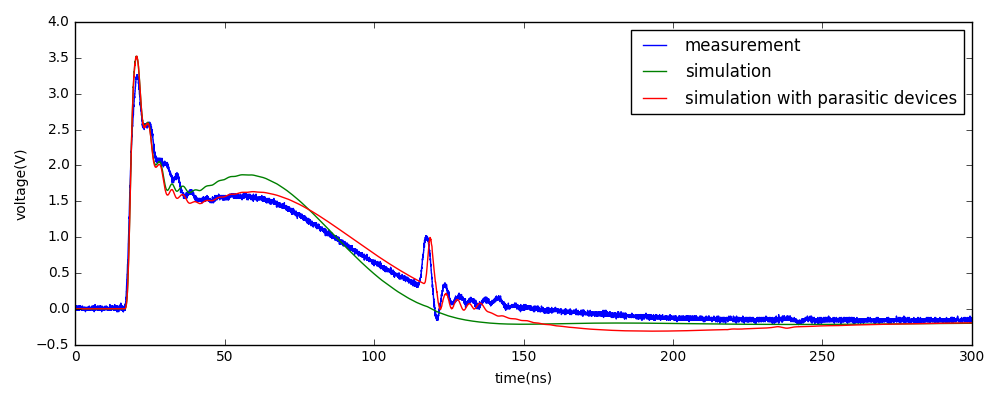
\includegraphics[width=0.95\textwidth]{src/5/figures/tlp_hmm_waveforms.png}
  \caption{Measurement versus simulation of a 250V TLP-HMM (equivalent 1kV HMM) on 2\textOmega{}}
  \label{fig:tlp_hmm_waveforms}
\end{figure}

\begin{table}[!h]
\centering
\begin{tabular}{@{}llll@{}}
\toprule
         & Standard (A)    & Measured (A)  & Simulated (A) \\ \midrule
peak     & 3.75 \pm 0.375  & 3.26          & 3.52 \\
30 ns    & 2 \pm 0.6       & 1.54          & 1.8  \\
60 ns    & 1 \pm 0.3       & 1.18          & 1.32 \\ \bottomrule
\end{tabular}
\caption{Measured and simulated currents versus standardized values}
\label{tab:mes-sim-std-currents}
\end{table}

% Analyse the curve
Overall, simulation and measurement correlate quite well.
There is a small difference for the slopes between 40ns and 150ns.
Investigation showed this difference comes from the shaping filter, and the inductances in particular.
Their frequency behavior is not as good as expected.
Having four inductances in parallel increases further this issue.
In the current shaping filter configuration, the parasitic capacitance of each inductor are in parallel.
They add up together, leading to a degraded frequency behavior.
For the next iteration of the shaping filter, a single RF inductor should be used instead.
The shaping filter model can be corrected by connecting in parallel a total parasitic capacitance of 2nF in series with a 15\textOmega{} parasitic resistor.

\begin{figure}[!h]
  \centering
  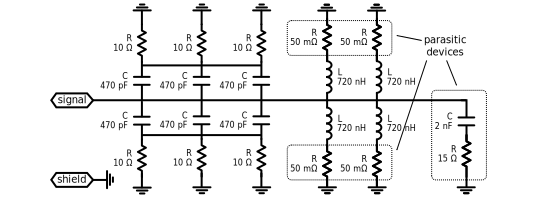
\includegraphics[width=0.8\textwidth]{src/5/figures/shaping_filter_schematic_parasitics.pdf}
  \caption{shaping-filter schematic with parasitics}
  \label{fig:shaping_filter_schematic_parasitics}
\end{figure}

The glitch visible at approximately 120 ns is due to the absorber, because of two different parasitic devices.
At the beginning of the TLP pulse, the parasitic capacitance between signal and ground is charged.
Using the simulation, it is estimated at 20 pF.
Its sudden discharge at the end of the TLP pulse causes the short voltage and current increase observed at 120 ns.
The parasitic series inductance of the three 2.2nF capacitors and the 50\textOmega{} resistor (Fig. \ref{fig:absorber_schematic_parasitics}) is responsible afterward for the small oscillation observed between 120 ns to 150 ns.
This issue should be fixed in the next iteration of the absorber by building the absorber on a dedicated PCB with 50\textOmega{} lines.
Guarantying matching along the path should eliminate this ringing oscillation.

\begin{figure}[!h]
  \centering
  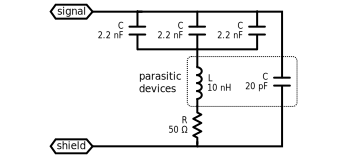
\includegraphics[width=0.5\textwidth]{src/5/figures/absorber_schematic_parasitics.pdf}
  \caption{absorber schematic with parasitics}
  \label{fig:absorber_schematic_parasitics}
\end{figure}

% TODO: Do next ?
% Afterwards, resistive loads of 2 10 and 0 are tested
% The first two loads are simply constituted of several resistors in parallel.
% The oscilloscope input impedance is used for the 50  load.
% In this case, reflections are eliminated by the matched load and the waveform is less disturbed.

% For 2 and 10, the measurements (Fig. 16 & 17) are quite noisy because of reflections.
% Despite that, it is interesting to observe that overall the amplitudes match well.
% The differences come mostly from parasitic devices not taken into account in those simulation.
%TODO: Waveforms 2ohm, 10ohm, 50ohms


\subsection{Comparison with an ESD Gun}
%TODO: Make a structural review of this section

Destroying ESD protections is actually a well known an common method for correlating stress generators (TODO: Find a reference).

Different ESD protections are tested until breakdown.
The goal is see if a mathematical relation can be established between failures levels found with each generator.

The test procedure is standard and consists in monitoring the leakage current after each new pulse.
Failure levels are compared for TLP, TLP-HMM and HMM.
Five samples are tested for each structure with each generator to ensure that the failure levels do not have large variations in failure levels. This number of samples is still quite low, but is considered sufficient for this study.
The results are summarized in Table 4.

%TODO: Table of failures
